% Credits are indicated where needed. The general idea is based on a template by Vel (vel@LaTeXTemplates.com) and Frits Wenneker.
%\documentclass[UTF8]{ctexart}
\documentclass[11pt, letterpaper]{article} % General settings in the beginning (defines the document class of your paper)
% 11pt = is the font size
% A4 is the paper size
% “article” is your document class
\usepackage{titling}
\usepackage{titlesec}
\setlength{\droptitle}{-3cm}

%----------------------------------------------------------------------------------------
%	Packages
%----------------------------------------------------------------------------------------
\usepackage[UTF8]{ctex}
% Necessary
\usepackage[german,english]{babel} % English and German language
\usepackage{caption}
\usepackage{booktabs} % Horizontal rules in tables
% For generating tables, use “LaTeX” online generator (https://www.tablesgenerator.com)
\usepackage{comment} % Necessary to comment several paragraphs at once
%\usepackage[utf8]{inputenc} % Required for international characters
\usepackage[T1]{fontenc} % Required for output font encoding for international characters
\usepackage{listings}
% Might be helpful
\usepackage{amsmath,amsfonts,amsthm} % Math packages which might be useful for equations
\usepackage{tikz} % For tikz figures (to draw arrow diagrams, see a guide how to use them)
\usepackage{tikz-cd}
\usetikzlibrary{positioning,arrows} % Adding libraries for arrows
\usetikzlibrary{decorations.pathreplacing} % Adding libraries for decorations and paths
\usepackage{tikzsymbols} % For amazing symbols ;) https://mirror.hmc.edu/ctan/graphics/pgf/contrib/tikzsymbols/tikzsymbols.pdf
\usepackage{blindtext} % To add some blind text in your paper
\usepackage{xcolor}


%---------------------------------------------------------------------------------
% Additional settings
%---------------------------------------------------------------------------------

%---------------------------------------------------------------------------------
% Define your margins
\usepackage{geometry} % Necessary package for defining margins

\geometry{
	top=2cm, % Defines top margin
	bottom=2cm, % Defines bottom margin
	left=2.2cm, % Defines left margin
	right=2.2cm, % Defines right margin
	includehead, % Includes space for a header
	%includefoot, % Includes space for a footer
	%showframe, % Uncomment if you want to show how it looks on the page
}

\setlength{\parindent}{15pt} % Adjust to set you indent globally

%---------------------------------------------------------------------------------
% Define your spacing
\usepackage{setspace} % Required for spacing
% Two options:
\linespread{1.5}
%\onehalfspacing % one-half-spacing linespread

%----------------------------------------------------------------------------------------
% Define your fonts
\usepackage[T1]{fontenc} % Output font encoding for international characters
\usepackage[utf8]{inputenc} % Required for inputting international characters

\usepackage{XCharter} % Use the XCharter font


%---------------------------------------------------------------------------------
% Define your headers and footers

\usepackage{fancyhdr} % Package is needed to define header and footer
\pagestyle{fancy} % Allows you to customize the headers and footers

%\renewcommand{\sectionmark}[1]{\markboth{#1}{}} % Removes the section number from the header when \leftmark is used

% Headers
\lhead{} % Define left header
\chead{\textit{}} % Define center header - e.g. add your paper title
\rhead{} % Define right header

% Footers
\lfoot{} % Define left footer
\cfoot{\footnotesize \thepage} % Define center footer
\rfoot{ } % Define right footer

%---------------------------------------------------------------------------------
%	Add information on bibliography
\usepackage{natbib} % Use natbib for citing
\usepackage{har2nat} % Allows to use harvard package with natbib https://mirror.reismil.ch/CTAN/macros/latex/contrib/har2nat/har2nat.pdf

% For citing with natbib, you may want to use this reference sheet:
% http://merkel.texture.rocks/Latex/natbib.php

%---------------------------------------------------------------------------------
% Add field for signature (Reference: https://tex.stackexchange.com/questions/35942/how-to-create-a-signature-date-page)
\newcommand{\signature}[2][5cm]{%
  \begin{tabular}{@{}p{#1}@{}}
    #2 \\[2\normalbaselineskip] \hrule \\[0pt]
    {\small \textit{Signature}} \\[2\normalbaselineskip] \hrule \\[0pt]
    {\small \textit{Place, Date}}
  \end{tabular}
}

\renewcommand{\abstractname}{摘要}
%---------------------------------------------------------------------------------
%	General information
%---------------------------------------------------------------------------------
%\begin{comment}
\title{Project Report} % Adds your title
\author{
Qi Gao \big(qxg150130@utdallas.edu\big)\\
Pancham Mamania \big(pxm172730@utdallas.edu\big)
 % Add your first and last name
    %\thanks{} % Adds a footnote to your title
    %\institution{YOUR INSTITUTION} % Adds your institution
  }

\date{05/08/2019} % Adds the current date to your “cover” page; leave empty if you do not want to add a date
%\end{comment}

%---------------------------------------------------------------------------------
%	Define what’s in your document
%---------------------------------------------------------------------------------
\definecolor{light-gray}{gray}{0.95}

\begin{document}
\lstset{%numbers=left,
%numberstyle=\tiny,
keywordstyle=\color{blue!70},
commentstyle=\color{red!50!green!50!blue!50},
backgroundcolor=\color{light-gray},
%frame=shadowbox,
rulesepcolor=\color{red!20!green!20!blue!20},
breaklines=true,
extendedchars=true
}

% If you want a cover page, uncomment "%---------------------------------------------------------------------------------
% Cover page
%---------------------------------------------------------------------------------

% Here are more templates for other cover pages: https://www.latextemplates.com/cat/title-pages

% This example is based on this cover page example: https://www.latextemplates.com/template/academic-title-page

\begin{titlepage} % Starts new environment where the page number is not displayed and the count starts at 1 for the next page

%------------------------------------------------
%	Institutional information
%------------------------------------------------
	
\begin{minipage}{0.4\textwidth} % Begins new environment (like a text box)
    \begin{flushleft} % Sets environment on the left side of the paper
    \large
    University of XX\\ % Add your institution
    Chair of Political Science IV\\ % Add the chair
    Fall 2018\\ % Add term
    COURSE TITLE\\ % Add course title
    Supervisor: NAME % Add instructor/supervisor name 
    \end{flushleft}
\end{minipage}
	
\vspace*{2in} % Adds some space in-between
	
\center % Centre everything on the page

%------------------------------------------------
%	Main part
%------------------------------------------------
	
{\huge\bfseries TITLE OF YOUR PAPER}\\[0.4cm] % Add your paper title 
{\large\today}\\[0.4cm] % Add date (current day)
FIRSTNAME LASTNAME % Add your name
	
\vfill % Adds additional space

%------------------------------------------------
%	General information about the author
%------------------------------------------------

\vfill % Adds additional space

Your contact info \\ % Add your contact info
Your Program \\ % Add info about your program
Semester you are enrolled \\ % Add info about your semester

\vfill % Adds additional space

%------------------------------------------------
%	Word count
%------------------------------------------------

\vfill % Adds additional space
	
Word count: XXXX % To indicate the word count
% How to check words in a LaTeX document: https://www.overleaf.com/help/85-is-there-a-way-to-run-a-word-count-that-doesnt-include-latex-commands
	

	
\end{titlepage}" and uncomment "\begin{comment}" and "\end{comment}" to comment the following lines
%%---------------------------------------------------------------------------------
% Cover page
%---------------------------------------------------------------------------------

% Here are more templates for other cover pages: https://www.latextemplates.com/cat/title-pages

% This example is based on this cover page example: https://www.latextemplates.com/template/academic-title-page

\begin{titlepage} % Starts new environment where the page number is not displayed and the count starts at 1 for the next page

%------------------------------------------------
%	Institutional information
%------------------------------------------------
	
\begin{minipage}{0.4\textwidth} % Begins new environment (like a text box)
    \begin{flushleft} % Sets environment on the left side of the paper
    \large
    University of XX\\ % Add your institution
    Chair of Political Science IV\\ % Add the chair
    Fall 2018\\ % Add term
    COURSE TITLE\\ % Add course title
    Supervisor: NAME % Add instructor/supervisor name 
    \end{flushleft}
\end{minipage}
	
\vspace*{2in} % Adds some space in-between
	
\center % Centre everything on the page

%------------------------------------------------
%	Main part
%------------------------------------------------
	
{\huge\bfseries TITLE OF YOUR PAPER}\\[0.4cm] % Add your paper title 
{\large\today}\\[0.4cm] % Add date (current day)
FIRSTNAME LASTNAME % Add your name
	
\vfill % Adds additional space

%------------------------------------------------
%	General information about the author
%------------------------------------------------

\vfill % Adds additional space

Your contact info \\ % Add your contact info
Your Program \\ % Add info about your program
Semester you are enrolled \\ % Add info about your semester

\vfill % Adds additional space

%------------------------------------------------
%	Word count
%------------------------------------------------

\vfill % Adds additional space
	
Word count: XXXX % To indicate the word count
% How to check words in a LaTeX document: https://www.overleaf.com/help/85-is-there-a-way-to-run-a-word-count-that-doesnt-include-latex-commands
	

	
\end{titlepage}

%\begin{comment}
\maketitle % Print your title, author name and date; comment if you want a cover page

%\begin{center} % Center text
    %Word count: XXXX
% How to check words in a LaTeX document: https://www.overleaf.com/help/85-is-there-a-way-to-run-a-word-count-that-doesnt-include-latex-commands
%\end{center}
%\end{comment}

%----------------------------------------------------------------------------------------
% Introduction
%----------------------------------------------------------------------------------------
\section*{Preface}
The tokens we picked are Tierion, Aragon, and Bitqy. Because we cannot find token126, hms and lino in token pirce folder, so we moved down and picked Bitqy as our third token. Because of limited space, we only present graph and parameters of one token that is Tierion. However, the three tokens has no much difference with other, one of the things need to take care is to convert the data type and remove outliers. In addition, some explainations and findings are in comments among the code.
\setcounter{page}{1} % Sets counter of page to 1
\section{Ethereum and Tokens Description} % Add a section title
\subsection{Ethereum and ERC20} % Add a subsection
Ethereum is an innovation that applies some of the technologies and concepts of Bitcoin in computing. Bitcoin is considered a system that maintains a shared global book that securely records all bitcoin bills. Ethereum uses a number of mechanisms similar to Bitcoin (such as blockchain technology and P2P networks) to maintain a shared computing platform that can flexibly and safely run any program the user wants.

\subsection{Project Tokens}  % Add another subsection
\subsubsection{Tierion}
Tierion is building a common data validation platform. Tierion's working principle is simply to create a proof that associates data with transactions on a blockchain. This process is called "anchoring." Anyone with this proof can verify the integrity and time stamp of the data without relying on any trusted authority.

\subsubsection{Aragon}
Aragon's decentralized APP on the Ethereum blockchain allows anyone to create and manage any organization. It implements the basic functions of shareholder roster, token transfer, voting, job appointment, financing, and accounting. It can be defined by modifying the charter. The behavior of organizations on the chain provides opportunities to create and manage decentralized organizations.

\subsubsection{Bitqy}
Bitqy is also called BQ, which is the official cryptocurrency issued by Bitqyck. Bitqyck will use BQ to scan various cryptocurrencies, including bitcoin and full-service data support and management.


%----------------------------------------------------------------------------------------
% Literature review
%----------------------------------------------------------------------------------------

\section{Project Goal}
This project has two parts. The first goal is to filter out all outliers from each tokens and then find out the best distribution for each token. The second part is that we find out the best K that is the number of most active buyers, which bought most tokens or has most number of transactions. And the top K buyers' data gives the best fitted multiple regression model.

\section{Question 1}
First of all, we read data file and then filtered out all outliers which amount of tokens per transcation is larger than total supply.
\lstset{language=R}
\begin{lstlisting}
tierion <- read_delim('networktierionTX.txt', delim = " ", col_names = F)
names(tierion) <- c('fromID', 'toID', 'unixTime', 'tokenAmount')
decimals <- 10^8
supply <- 1 * 10^9
#filter out all outliers
tierionFiltered <-filter(tierion,tokenAmount < decimals * supply)
#Amount of users made those unnormal transcation and buys they made and remove those
tierion_outliers<- filter(tierion,tokenAmount >= decimals * supply)
user_outliers <- tierion_outliers %>% group_by(toID) %>% summarise(n = n()) %>% ungroup
number_users_outliers<-nrow(user_outliers)
#get top X buyers data
buys<-tierionFiltered%>% group_by(toID) %>% summarise(n = n()) %>% ungroup
buys_sorted_dec<-buys[order(-buys$n),]
#top 30 active buyers and number of buys
top_30_buyers<-buys_sorted_dec%>%head(30)

#####group by user pairs#####
#This for loop is to group by pairs of users. For example, pairs users like A->B and B->A would be seen a pair of address, and then sum up number of buys.
buys_pairs<-tierionFiltered%>% group_by(fromID, toID) %>% summarise(n = n()) %>% ungroup
for (row in 1:nrow(buys_pairs)) {
  a<-buys_pairs[row,"fromID"]
  b<-buys_pairs[row,"toID"]
  for (inner_row in row:nrow(buys_pairs)) {
    c<-buys_pairs[inner_row,"fromID"]
    d<-buys_pairs[inner_row,"toID"]
    if(a==d&&b==c){
      buys_pairs[inner_row,"fromID"]<-d
      buys_pairs[inner_row,"toID"]<-c
    }
  }
}
buys_pairs<-tierionFiltered%>% group_by(fromID, toID) %>% summarise(n = n()) %>% ungroup
#sort and get those buyers that their number of buys less than 30 that covers 98% of population, because this would make graph look better.
buys_pair_sorted_asc<-buys_pairs[order(buys_pairs$n),]
buys_pair_less_30<-subset(buys_pair_sorted_asc,n<30)
#####find out estimates of paramaters of for several distributions based on the buys_pairs data set#####
exp_dis <- fitdist(buys_pair_less_30$n, 'exp')
gamma_dis <- fitdist(buys_pair_less_30$n, 'gamma')
lnorm_dis <- fitdist(buys_pair_less_30$n, 'lnorm')
pois_dis <- fitdist(buys_pair_less_30$n, 'pois')
weibull_dis <- fitdist(buys_pair_less_30$n, 'weibull')
######################draw graph#######################
#Finally, draw the density graph, then we plug in those parameters we got in stat_function and plot those on top of it. The red line is lognormal function, blue line is gamma function, green is exponential function, yellow line is weibull function and orange line is possion function.
all_density <- ggplot(data=buys_pair_less_30) +
  geom_histogram(bins=30,aes(x = buys_pair_less_30$n, ..density..)) +
  stat_function(fun = dlnorm, args = list(meanlog = 0.2373987, sdlog = 0.4791316), colour = "red")+
  stat_function(fun = dgamma, args = list(shape = 3.020395, rate=2.000602), colour = "blue")+
  stat_function(fun=dexp, args=list(rate=0.6623558),colour="green")+
  stat_function(fun=dweibull, args=list(shape=1.360851, scale=1.678697),colour="yellow")+
  stat_function(fun=dpois, args=list(lambda=1.509763),colour="orange")+  xlab("No.Buys")
all_density
\end{lstlisting}


\subsection*{Conclusion of Question 1}
As the graph shows to us, lognormal distribution intuitively fits the pair users distribution best. We can explain that by common sense that is most user pairs only trade once or few times to each other because they trade on platforms and they do not know each other. In addition, most platform do matchmaking trading system and identity anonymous. So that is why majority of pair of traders only trade once with each other.
The parameters I used of lognormal distribution is as follows:
\lstset{language=R}
\begin{lstlisting}
> lnorm_dis
Fitting of the distribution ' lnorm ' by maximum likelihood
Parameters:
         estimate   Std. Error
meanlog 0.1931520 0.0014032182
sdlog   0.4427993 0.0009922024
\end{lstlisting}

\begin{figure}[ht]

\centering
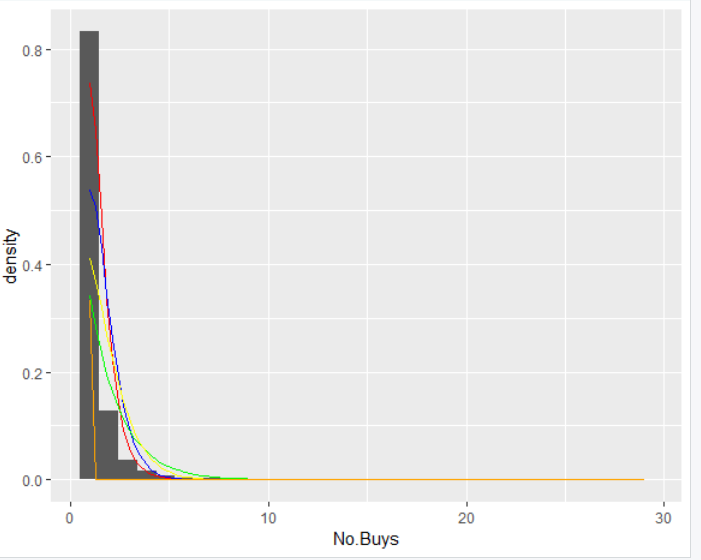
\includegraphics[scale=0.7]{Q1_graph.PNG}
\label{fig:label}
\end{figure}

\begin{comment}
\begin{figure}[htbp]
\begin{minipage}[t]{0.3\textwidth}
\centering
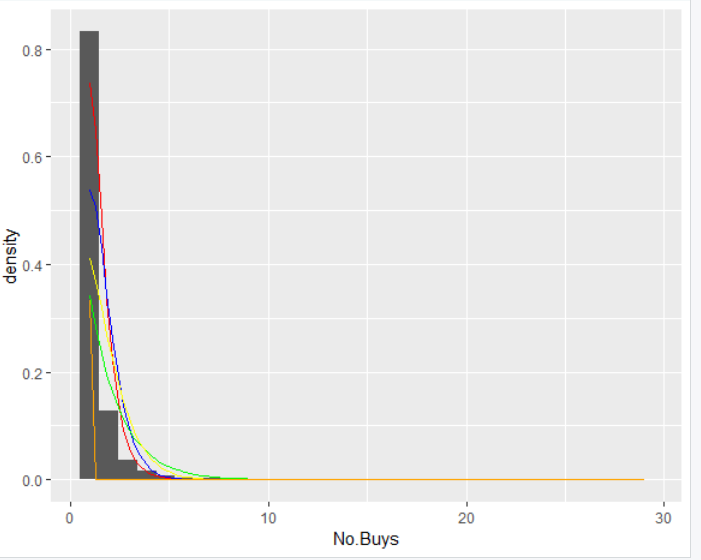
\includegraphics[width=\textwidth]{Q1_graph.PNG}
%\caption{Q1 graph}
\end{minipage}
\begin{minipage}[t]{0.3\textwidth}
\centering
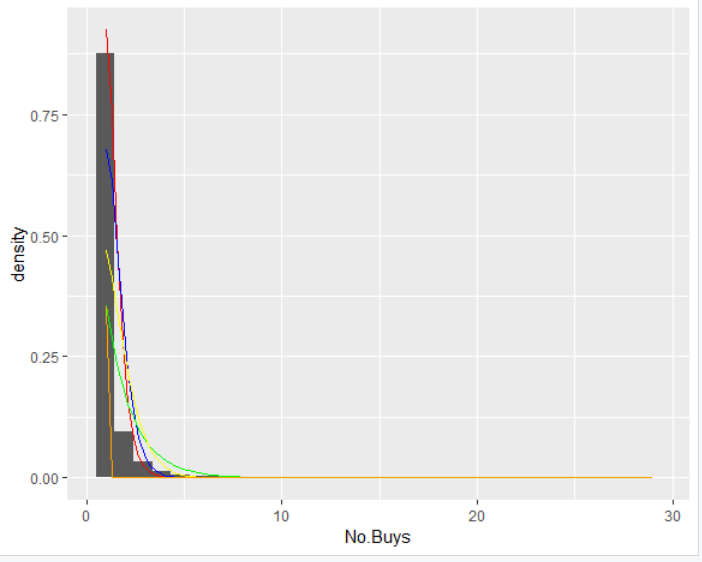
\includegraphics[width=\textwidth]{Q1_graph_2.PNG}
%\caption{Q1 graph_2.PNG}
\end{minipage}
\begin{minipage}[t]{0.3\textwidth}
\centering
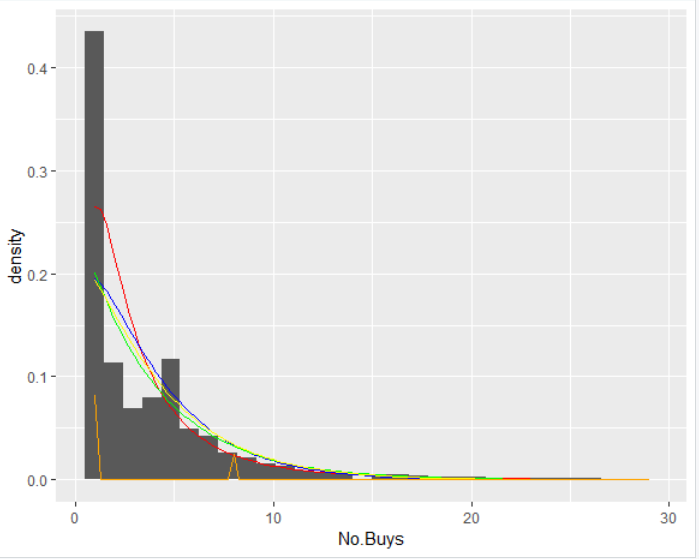
\includegraphics[width=\textwidth]{Q1_graph_3.PNG}
%\caption{Q1 graph_3.PNG}
\end{minipage}
\end{figure}
\end{comment}
\section{Question 2}
\begin{lstlisting}
#####################Question2################
#We have omitted some code because of limited space.The omitted part is about loading data and adjusting type of value.
## merge the prices and edge
tierion_merged<-merge(x = tierion_prices, y = tierion_filtered, by = "date", all.x = TRUE)
################Determin K##########################
#The following loop is to determin best K in the top active buyers which ranks by amount of tokens of all transcations. Here we choose top 30 as the first round, if the parameters is not that good, then try top 100, 200 and so on. This loop generates graphs and parameters for every top 30 buyers and we can analyze those information to figure out conclusion.
top_30_buyers<-buys_sorted_dec%>%head(30)
top_K<-c(1:30)
count <- 1
for (val in top_K) {
  top_K_buyers<-buys_sorted_dec%>%head(val)
  #filter out top K active buyers data
  filter_K_tierion_merged<-filter(tierion_merged,toID %in% top_K_buyers$toID)
  #take the average price of open and close price filter_K_tierion_merged=transform(filter_K_tierion_merged,average_price= (Open+Close)/2)
  filter_K_tierion_merged$num_Date <-  as.numeric(as.POSIXct(filter_K_tierion_merged$date))
  #This is an important step. This is to group data by date, and sum up tokenAmount, take average of Close price of top K buyers made in same date, those data will be used later.
  filered<-filter_K_tierion_merged%>% group_by(num_Date) %>% summarise(n = n(),Close=mean(Close),tokenAmount=sum(tokenAmount),average_price=mean(average_price))
  #shift down Close price by one day in order to use the Close price as outcome that is price of next day.
  shift <- function(x, n){
    c(x[-(seq(n))], rep(NA, n))
  }
  filered$new_Close<-shift(filered$Close,1)
  num_rows<-nrow(filered)
  filered[-num_rows,]
  #fit data in multiple regression model
  regression<-lm(filered$new_Close~filered$tokenAmount+filered$n+filered$average_price)
  #export paramaters and graph to local
  setwd("C:/Users/ygaoq/Desktop/Tierion")
  yourfilename=paste("W",val,".txt",sep="")
  capture.output(summary(regression),append = TRUE,file = "Final_Result.txt")
  summary(regression)
  par(mfcol=c(2,2))
  setwd("C:/Users/ygaoq/Desktop/Tierion")
  yourfilename=paste("A",val,".png",sep="")
  png(file=yourfilename)
  opar <- par(mfrow=c(2,2))
  plot(regression)
  dev.off()
}
########Parameters of Best K###########
Call:
lm(formula = filered$new_Close ~ filered$tokenAmount + filered$n + filered$Open)
Residuals:
      Min        1Q    Median        3Q       Max
-0.088209 -0.009052 -0.003640  0.007277  0.206146
Coefficients:
                      Estimate Std. Error t value Pr(>|t|)
(Intercept)          8.758e-03  3.390e-03   2.584   0.0104 *
filered$tokenAmount -5.103e-19  2.308e-18  -0.221   0.8252
filered$n            3.633e-06  8.994e-06   0.404   0.6866
filered$Open         9.201e-01  2.447e-02  37.599   <2e-16 ***
---
Signif. codes:  0 ‘***’ 0.001 ‘**’ 0.01 ‘*’ 0.05 ‘.’ 0.1 ‘ ’ 1
Residual standard error: 0.02653 on 248 degrees of freedom
  (1 observation deleted due to missingness)
Multiple R-squared:  0.8571,	Adjusted R-squared:  0.8554
F-statistic: 495.8 on 3 and 248 DF,  p-value: < 2.2e-16
\end{lstlisting}

\begin{figure}[htbp]
\begin{minipage}[t]{0.5\textwidth}
\centering
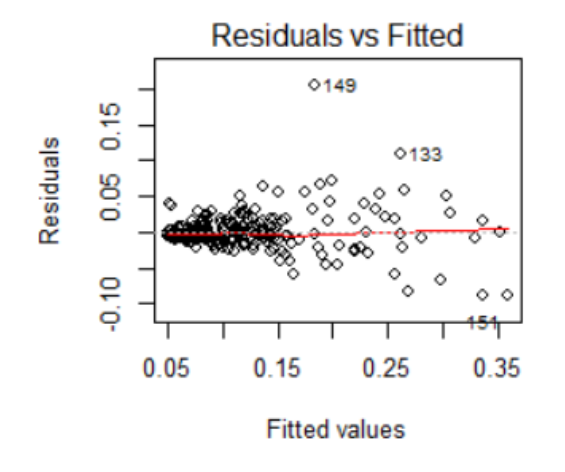
\includegraphics[width=\textwidth]{Capture1.PNG}
%\caption{Q1 graph}
\end{minipage}
\begin{minipage}[t]{0.5\textwidth}
\centering
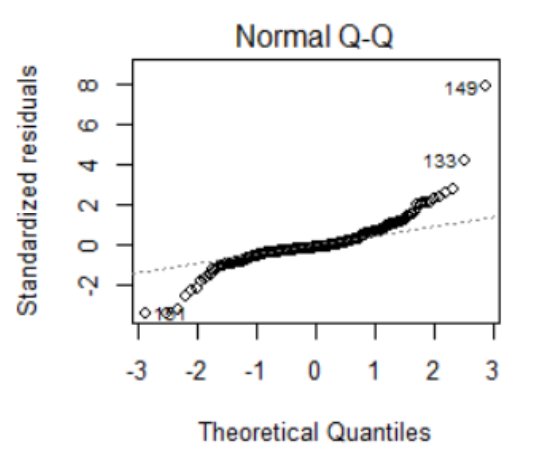
\includegraphics[width=\textwidth]{Capture2.PNG}
%\caption{Q1 graph_2.PNG}
\end{minipage}
\end{figure}

\subsection*{Conclusion of Question 2}
The process of determining best regressors is very difficult. Finally, we choose today's average price of open and close price, total token amount from every top K buyer, number of transcations as regressors, and pick Close price from next date as outcome. Next, fit those data in regression model and export every parameters output and graphs to local in order to figure out the best K. So, finally we have 30 graphs and groups of parameters in local for each token. From the parameters and graphs we have and compare them one by one, the best K is about after 15, which means there is almost no difference in increasing K after 15. Different token has different best K, the best K of aragon is 13 and best K of bitqy is 16. First of all, let us look at adjusted R-squared that is more useful than normal R-squared. When K increases to 15, the adjusted R-squared remains at around 0.8554, which is decent number for regression model. And let's analyze the four graphs above.

Residual and fitting values on the left side, the data points between the residual and the fitted values are evenly distributed on both sides of y=0, showing a random distribution, and the red line presents a smooth curve with no obvious shape features.
The residual QQ map on the right side, the data points are arranged in a diagonal line, tending to a straight line, and are directly passed diagonally, which intuitively conforms to the normal distribution.

\end{document}
